\documentclass[11pt,a4j]{jsarticle}
\usepackage{ascmac}
\usepackage{amsmath}
\usepackage[dvipdfmx]{graphicx}
\usepackage{upgreek}

\newsavebox{\circlebox}
\savebox{\circlebox}{\fontencoding{OMS}\selectfont\Large\char13}
\newlength{\circleboxwdht}
\newcommand{\centercircle}[1]{%
  \setlength{\circleboxwdht}{\wd\circlebox}%
  \addtolength{\circleboxwdht}{\dp\circlebox}%
  \raisebox{0.4\dp\circlebox}{%
    \parbox[][\circleboxwdht][c]{\wd\circlebox}{\centering#1}}%
  \llap{\usebox{\circlebox}}%
}	%丸数字(文字)環境。\centercircle{入れたい文字} で丸文字を表示する。





\title{宮島研究室2019年度B4スタート実験}
\author{宮島研究室B4 渡辺慧}
\date{\today}

\begin{document}

\maketitle %タイトル

%\newpage

%\tableofcontents %目次



%%\listoffigures%図目次。確認用。後で消す

\newpage
\section{本研究の目的}
本研究の目的は、物質の光学反応を観測する際に用いる分光計を正しく取り扱い、CdS、GaAs及びGaAs/AlGaAs量子井戸の発光の特性を測定することである。

\newpage
\section{光学系の扱い及び半導体の発光特性}

\subsection{光学系の要素}
\subsubsection{分光器}

分光器は、光を波長ごとに分散させ、任意の波長の光を取り出す装置である。分光器の概略図を図%\ref{fig_monochro1}に示す。入射スリットから入射した光を分散素子に照射し、分散した光のうち取り出したい波長のものだけを出射スリットから出射させることで、分光を行っている。出射スリットから出た光を受光素子に照射することで、入射した光のスペクトルを得ることができる。
今回の実験で用いた分光器では、分散素子に反射型回折格子、受光素子にCCD(電荷結合素子、Chage Coupled Device)を用いた。

\begin{figure}[h]
	\centering
	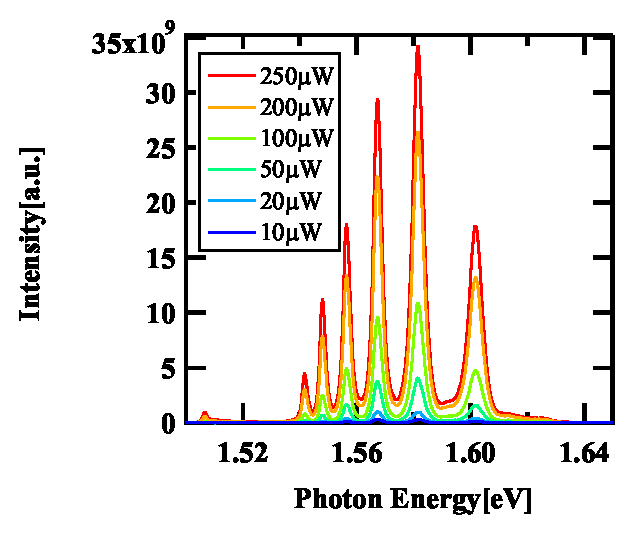
\includegraphics[clip]{mqw_77_spec.eps}
	\caption{シングルモノクロメーター概略図.}
	\label{fig_monochro1}
\end{figure}



\end{document}
